\section{Data}
\label{sec:data}

% DRAFT by Claude (13 Oct 2026), written from the pipeline code and the
% final results (docs/NEXT_STEPS.md section 1a; results/t1_all/DATA_CARD.md).
% Brian: rewrite it in your own words, and disclose the AI assistance
% (CSE 5999 and IEEE both require it).
\todo{Draft by Claude: rewrite in your own words.}

\textbf{Sources.} We use public GPS traces uploaded to
OpenStreetMap (OSM)~\cite{osm} in 17 mountain regions of the United States
and Canada (Fig.~\ref{fig:map}), chosen for relief, trail density and lidar
coverage. The traces come from three sources: the OSM trackpoints API,
which returns the timestamped points of identifiable and trackable uploads
tile by tile; the original GPX files of identifiable uploads, which give
whole hikes at the device's own sampling; and a crawl of 1.5 million
original files of public and identifiable uploads from 2016--2022, which
keeps the timestamps the API drops. Sixteen regions combine all three; the
Bay Area uses the crawl only, because the API times out on its tiles.

\textbf{Processing.} Each recording is cleaned (repeated timestamps,
steps faster than 60~km/h), split at gaps over 5~min and thinned to points
at least 5~s apart. A step counts as a stop when the point 60~s later lies
within 10~m. Traces are map-matched to the OSM trail and road network with
a hidden Markov model~\cite{newson2009hidden} (97\% of points matched), and
the matched path is cut into 50~m segments. Each segment records its moving
speed, its signed slope along the direction of travel from the 5~m USGS
3DEP elevation grid~\cite{sugarbaker2017status} (resampled from 1~m lidar
under at least 83\% of walked trail in 13 regions), the OSM tags of its way
and the trace's recording interval. Duplicate uploads are removed, and
traces that start within 15~min and 1~km of each other form one outing (a
group hike), the unit we resample. Travel mode is inferred per trace,
anchored on trails closed to bikes and horses. Against the activity that
327 uploaders' apps wrote into their files, 93\% of labelled hikes are
classed as walking, and 5\% of the labelled traces we class as walking say
bike or ski.

\textbf{The dataset.} The regions hold 2,876 hiking traces. The walking
analysis set (walking traces on trails) has 290,640 segments (14,532~km)
from 2,046 traces in 1,992 outings and 4,702 moving hours. Its uploaders are
OSM mappers and enthusiasts rather than a random sample of hikers, and busy
API tiles do not reach their oldest uploads. Traces logged more than 10~s
apart read up to 11\% slow, because straight lines between points cut
corners and short stops hide between them; the gains we report are the
same at every recording rate (Sec.~\ref{sec:results}).

\begin{figure}[t]
\centering
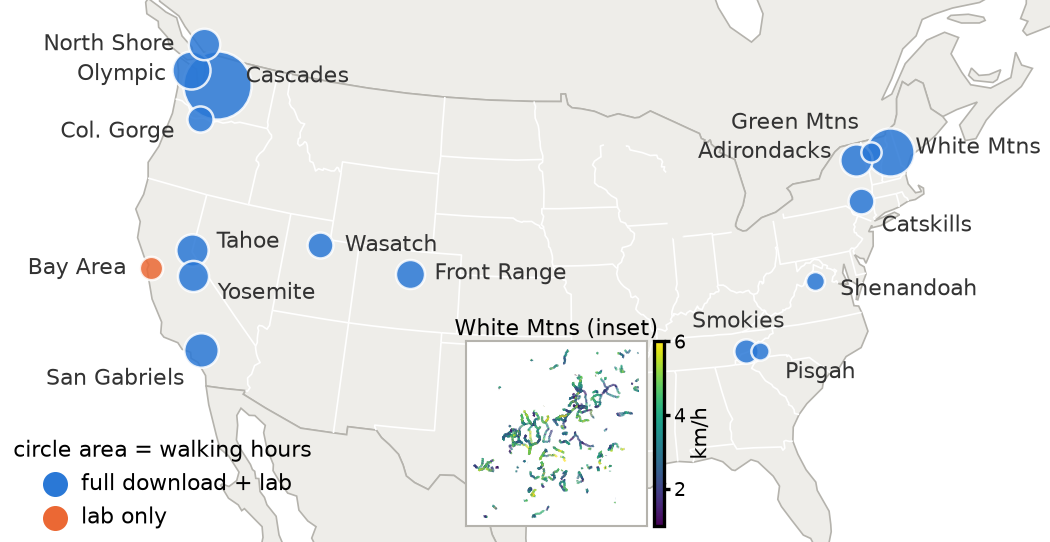
\includegraphics[width=\columnwidth]{fig_map}
\caption{The 17 regions. Circle area is walking hours (1,992 outings,
4,702 h in total). Blue: full OSM download plus the lab crawl; orange: lab
crawl only. Inset: the White Mountains' 34,535 walking segments colored by
speed.}
\label{fig:map}
\end{figure}
